\section{Лекция 8. Интегрирующий множитель}
\noeqref{eq:l8_nonexact_ode, eq:l8_ineq_ exact, eq:l8_du_mu, eq:l8_ex1}
\noeqref{eq:l8_sys_dxdy, eq:l8_det_zero, eq:l8_mu_explicit, eq:l8_pde_mu}
\noeqref{eq:l8_cond_mux, eq:l8_form_mux, eq:l8_cond_muy, eq:l8_form_muy}
\noeqref{eq:l8_cond_muw, eq:l8_form_muw, eq:l8_split_ode, eq:l8_split_mu}
\noeqref{eq:l8_f195}

\begin{flushright}
    20.10.26
\end{flushright}

\subsection{Понятие интегрирующего множителя}

Рассмотрим дифференциальное уравнение 1-го порядка в симметричной
дифференциальной форме в односвязной области $D \subset \R^2$:
\begin{equation} \label{eq:l8_nonexact_ode}
    M(x, y) \, dx + N(x, y) \, dy = 0, \tag{1}
\end{equation}
где коэффициенты непрерывно дифференцируемы: $M, N \in C^1(D)$ (то есть
$M, N, M'_x, M'_y, N'_x, N'_y \in C(D)$).

Предположим, что в области $D$ критерий полного дифференциала из Лекции 7
(Теорема~\ref{thm:l7_criterion}) \textbf{не выполняется}:
\begin{equation} \label{eq:l8_ineq_ exact}
    \frac{\partial N}{\partial x} \neq \frac{\partial M}{\partial y}. \tag{2}
\end{equation}
В этом случае левая часть уравнения \eqref{eq:l8_nonexact_ode} не является
полным дифференциалом никакой функции, однако уравнение нередко удаётся свести
к уравнению в полных дифференциалах путём умножения обеих частей на специально
подобранную функцию $\mu(x, y) \not\equiv 0$.

\begin{definition}
    Ненулевая функция $\mu(x, y) \in C^1(D)$ (то есть
    $\mu, \mu'_x, \mu'_y \in C(D)$) называется \textdef{интегрирующим
    множителем} дифференциального уравнения \eqref{eq:l8_nonexact_ode}, если
    после умножения на неё левая часть уравнения обращается в полный
    дифференциал некоторой функции $u(x, y) \in C^1(D)$:
    \begin{equation} \label{eq:l8_du_mu}
        du(x, y) = \mu(x, y) M(x, y) \, dx + \mu(x, y) N(x, y) \, dy = 0.
        \tag{3}
    \end{equation}
    Если интегрирующий множитель $\mu(x, y)$ известен, то решение уравнения
    \eqref{eq:l8_nonexact_ode} записывается в виде общего интеграла
    $u(x, y) = C$.
\end{definition}

\begin{remark}[Геометрический смысл и проверка особых множеств] ~
    \begin{enumerate}
        \item \textbf{Геометрическая интерпретация.} В каждой точке
        $(x, y) \in D$, где $\mu(x, y) \neq 0$, вектор нового поля
        $(\mu M, \mu N)$ коллинеарен исходному вектору $(M, N)$. Поэтому
        умножение на $\mu(x, y)$ не меняет поля направлений и семейства
        интегральных кривых, но изменяет длины векторов так, чтобы векторное
        поле стало потенциальным: $(\mu M, \mu N) = \nabla u(x, y)$.
        \item \textbf{Приобретение и потеря решений.} При умножении уравнения
        \eqref{eq:l8_nonexact_ode} на $\mu(x, y)$ могут появиться посторонние
        решения (линии, на которых $\mu(x, y) = 0$), либо, напротив, могут
        быть потеряны решения, на которых функция $\mu(x, y)$ терпит разрыв.
        Такие кривые необходимо исследовать отдельно прямой подстановкой в
        исходное уравнение \eqref{eq:l8_nonexact_ode}.
    \end{enumerate}
\end{remark}

\begin{example}
    Решить с помощью интегрирующего множителя уравнение:
    \begin{equation} \label{eq:l8_ex1}
        y \, dx - x \, dy = 0. \tag{4}
    \end{equation}

    \begin{proof}[Решение]~\\
        \begin{quote}
            Здесь $M(x, y) = y$ и $N(x, y) = -x$, поэтому
            \[
                \frac{\partial M}{\partial y} = 1 \neq -1 =
                \frac{\partial N}{\partial x},
            \]
            и уравнение \eqref{eq:l8_ex1} не является уравнением в полных
            дифференциалах.

            Заметим, что при умножении уравнения на функцию
            $\mu(x, y) = \dfrac{1}{y^2}$ (при $y \neq 0$) левая часть
            сворачивается в полный дифференциал частного:
            \[
                \frac{y \, dx - x \, dy}{y^2} = d\left(\frac{x}{y}\right) = 0
                \implies \frac{x}{y} = C.
            \]
            Поскольку множитель $\mu(x, y) = \frac{1}{y^2}$ не определён на
            прямой $y = 0$, проверим $y = 0$ отдельно: подстановка $y = 0, \;
            dy = 0$ в исходное уравнение \eqref{eq:l8_ex1} обращает его в
            верное тождество $0 = 0$.

            \textbf{Ответ:} $\dfrac{x}{y} = C$, а также $y = 0$.
        \end{quote}
    \end{proof}
    
\end{example}

\begin{figure}[H]
    \centering
    \begin{tikzpicture}[scale=1.1]
        % Оси координат
        \draw[->] (-2.8, 0) -- (2.8, 0) node[right] {$x$};
        \draw[->] (0, -2.2) -- (0, 2.2) node[above] {$y$};

        % Особая (потерянная при делении на y^2) прямая y = 0
        \draw[red, very thick] (-2.6, 0) -- (2.6, 0)
            node[above left, red] {$y = 0$};

        % Семейство прямых x / y = C
        \foreach \ang/\lbl in {25/C_1, 55/C_2, 125/C_3, 155/C_4} {
            \draw[blue, thick] (\ang:-2.3) -- (\ang:2.3);
        }
        \node[blue, right] at (1.5, 1.8) {$\dfrac{x}{y} = C$};

        % Выколотая точка (0, 0), где пересекаются все линии уровня
        \fill[white] (0, 0) circle (2pt);
        \draw[black, thick] (0, 0) circle (2pt);
    \end{tikzpicture}
    \caption{Семейство интегральных кривых уравнения $y \, dx - x \, dy = 0$:
    прямые $x / y = C$ и прямая $y = 0$, на которой интегрирующий множитель
    $\mu = 1 / y^2$ терпит разрыв.}
\end{figure}

\vspace{1 em}

\begin{remark}
    Интегрирующий множитель определяется неоднозначно. Например, для уравнения
    $y \, dx - x \, dy = 0$ интегрирующими множителями также служат функции
    $\mu_2 = \dfrac{1}{x^2}$ (даёт $d\left(-\frac{y}{x}\right) = 0$),
    $\mu_3 = \dfrac{1}{x y}$ (даёт $d\left(\ln \abs{\frac{x}{y}}\right) = 0$) и
    $\mu_4 = \dfrac{1}{x^2 + y^2}$ (даёт $d\left(\arctan \frac{x}{y}\right) = 0$).
\end{remark}



\subsection{Теорема существования интегрирующего множителя}

\begin{theorem}[\textbf{О существовании интегрирующего множителя}]
    Если дифференциальное уравнение \eqref{eq:l8_nonexact_ode} имеет общий
    интеграл $u(x, y) = C$, где $u \in C^1(D)$ и частные производные $u'_x, u'_y$
    не обращаются в нуль одновременно в области $D$, то в этой области
    уравнение \eqref{eq:l8_nonexact_ode} имеет интегрирующий множитель.
\end{theorem}

\begin{proof}[Доказательство]~\\
    \begin{quote}
        Пусть соотношение $u(x, y) = C$ задаёт общий интеграл уравнения
        $M \, dx + N \, dy = 0$. Продифференцируем тождество $u(x, y) = C$:
        \[
            du = \frac{\partial u}{\partial x} \, dx +
            \frac{\partial u}{\partial y} \, dy = dC = 0 \implies
            \frac{\partial u}{\partial x} \, dx =
            -\frac{\partial u}{\partial y} \, dy.
        \]
        С другой стороны, выполняется
        уравнение $M \, dx + N \, dy = 0$ (или, после умножения на искомый
        множитель $\mu \neq 0$, уравнение $\mu M \, dx + \mu N \, dy = 0$).
        Объединяя оба равенства в систему линейных однородных алгебраических
        уравнений относительно дифференциалов $dx$ и $dy$:
        \begin{equation} \label{eq:l8_sys_dxdy}
            \begin{cases}
                \mu M \, dx + \mu N \, dy = 0, \\[1mm]
                \dfrac{\partial u}{\partial x} \, dx +
                \dfrac{\partial u}{\partial y} \, dy = 0,
            \end{cases} \tag{5}
        \end{equation}
        Заметим, что система \eqref{eq:l8_sys_dxdy} имеет нетривиальное
        решение $(dx, dy) \neq (0, 0)$ тогда и только тогда, когда её
        определитель равен нулю:
        \begin{equation} \label{eq:l8_det_zero}
            \begin{vmatrix}
                \mu M & \mu N \\[2mm]
                \dfrac{\partial u}{\partial x} & \dfrac{\partial u}{\partial y}
            \end{vmatrix} = 0 \iff
            \mu M \frac{\partial u}{\partial y} -
            \mu N \frac{\partial u}{\partial x} = 0. \tag{6}
        \end{equation}
        Сокращая на $\mu \neq 0$, получаем пропорциональность коэффициентов:
        \[
            M \frac{\partial u}{\partial y} = N \frac{\partial u}{\partial x}
            \implies \frac{1}{N(x, y)} \frac{\partial u}{\partial y} =
            \frac{1}{M(x, y)} \frac{\partial u}{\partial x}.
        \]
        Обозначим это общее отношение через функцию $\mu(x, y)$:
        \begin{equation} \label{eq:l8_mu_explicit}
            \mu(x, y) = \frac{1}{N(x, y)} \frac{\partial u}{\partial y} =
            \frac{1}{M(x, y)} \frac{\partial u}{\partial x}. \tag{7}
        \end{equation}
        Отсюда сразу следуют равенства $\mu M = \dfrac{\partial u}{\partial x}$
        и $\mu N = \dfrac{\partial u}{\partial y}$. Умножая исходное уравнение
        \eqref{eq:l8_nonexact_ode} на определённую формулой
        \eqref{eq:l8_mu_explicit} функцию $\mu(x, y)$, получаем:
        \[
            \mu(x, y) M(x, y) \, dx + \mu(x, y) N(x, y) \, dy =
            \frac{\partial u}{\partial x} \, dx +
            \frac{\partial u}{\partial y} \, dy = du(x, y) = 0.
        \]
        Следовательно, $\mu(x, y)$ является интегрирующим множителем уравнения
        \eqref{eq:l8_nonexact_ode}.
    \end{quote}
\end{proof}

\subsection{Методы нахождения интегрирующего множителя}

Пусть $\mu = \mu(x, y)$ — интегрирующий множитель уравнения
\eqref{eq:l8_nonexact_ode} в односвязной области $D \subset \R^2$. Тогда
уравнение
\[
    \underbrace{\mu(x, y) M(x, y)}_{P(x, y)} \, dx +
    \underbrace{\mu(x, y) N(x, y)}_{Q(x, y)} \, dy = 0
\]
является уравнением в полных дифференциалах в области $D$. По критерию полного
дифференциала из Лекции 7 (Теорема~\ref{thm:l7_criterion}) для
этого необходимо и достаточно выполнения тождества:
\[
    \frac{\partial Q}{\partial x} = \frac{\partial P}{\partial y} \iff
    \frac{\partial \left(\mu(x, y) N(x, y)\right)}{\partial x} =
    \frac{\partial \left(\mu(x, y) M(x, y)\right)}{\partial y}.
\]
Раскрывая частные производные произведений по правилу Лейбница:
\[
    \frac{\partial \mu}{\partial x} N + \mu \frac{\partial N}{\partial x} =
    \frac{\partial \mu}{\partial y} M + \mu \frac{\partial M}{\partial y},
\]
и группируя слагаемые с производными $\mu$ в левой части, получаем основное
дифференциальное уравнение в частных производных для определения $\mu(x, y)$:
\begin{equation} \label{eq:l8_pde_mu}
    \frac{\partial \mu}{\partial x} N - \frac{\partial \mu}{\partial y} M =
    \mu \left(\frac{\partial M}{\partial y} -
    \frac{\partial N}{\partial x}\right). \tag{8}
\end{equation}

Нахождение общего решения уравнения в частных производных \eqref{eq:l8_pde_mu}
сложнее решения исходного ОДУ, однако нам достаточно найти \textbf{хотя бы одно
частное ненулевое решение} $\mu(x, y)$. Рассмотрим четыре важнейших случая, в
которых уравнение \eqref{eq:l8_pde_mu} решается явно.

\subsubsection{Случай 1. Интегрирующий множитель зависит только от $x$: $\mu = \mu(x)$}

\begin{proposition}
    Уравнение \eqref{eq:l8_nonexact_ode} допускает интегрирующий множитель
    вида $\mu = \mu(x)$, зависящий только от переменной $x$, тогда и только
    тогда, когда выражение
    \begin{equation} \label{eq:l8_cond_mux}
        \phi(x) = \frac{\dfrac{\partial M}{\partial y} -
        \dfrac{\partial N}{\partial x}}{N(x, y)} \tag{9}
    \end{equation}
    зависит только от $x$ (не зависит от $y$). В этом случае интегрирующий
    множитель определяется формулой:
    \begin{equation} \label{eq:l8_form_mux}
        \mu(x) = C \cdot \exp\left(\int \frac{\dfrac{\partial M}{\partial y} -
        \dfrac{\partial N}{\partial x}}{N(x, y)} \, dx\right). \tag{10}
    \end{equation}
\end{proposition}

\begin{proof}[Вывод формулы]~\\
    \begin{quote}
        Если $\mu = \mu(x)$, то $\dfrac{\partial \mu}{\partial y} = 0$ и
        $\dfrac{\partial \mu}{\partial x} = \mu'(x)$. Подставляя это в основное
        уравнение \eqref{eq:l8_pde_mu}, получаем:
        \[
            \mu'(x) N = \mu \left(\frac{\partial M}{\partial y} -
            \frac{\partial N}{\partial x}\right) \implies
            \frac{\mu'(x)}{\mu(x)} =
            \frac{\dfrac{\partial M}{\partial y} -
            \dfrac{\partial N}{\partial x}}{N(x, y)}.
        \]
        Левая часть зависит только от $x$, поэтому равенство возможно тогда и
        только тогда, когда правая часть также не зависит от $y$. Интегрируя
        по $x$, находим:
        \[
            \int \frac{d\mu}{\mu} =
            \int \frac{\dfrac{\partial M}{\partial y} -
            \dfrac{\partial N}{\partial x}}{N} \, dx \implies
            \mu(x) = C \cdot e^{\int \phi(x) \, dx}.
        \]
    \end{quote}
\end{proof}

\subsubsection{Случай 2. Интегрирующий множитель зависит только от $y$: $\mu = \mu(y)$}

\begin{proposition}
    Уравнение \eqref{eq:l8_nonexact_ode} допускает интегрирующий множитель
    вида $\mu = \mu(y)$, зависящий только от переменной $y$, тогда и только
    тогда, когда выражение
    \begin{equation} \label{eq:l8_cond_muy}
        \psi(y) = \frac{\dfrac{\partial M}{\partial y} -
        \dfrac{\partial N}{\partial x}}{M(x, y)} \tag{11}
    \end{equation}
    зависит только от $y$ (не зависит от $x$). В этом случае интегрирующий
    множитель определяется формулой:
    \begin{equation} \label{eq:l8_form_muy}
        \mu(y) = C \cdot \exp\left(-\int \frac{\dfrac{\partial M}{\partial y} -
        \dfrac{\partial N}{\partial x}}{M(x, y)} \, dy\right). \tag{12}
    \end{equation}
\end{proposition}

\begin{proof}[Вывод формулы]~\\
    \begin{quote}
        Если $\mu = \mu(y)$, то $\dfrac{\partial \mu}{\partial x} = 0$ и
        $\dfrac{\partial \mu}{\partial y} = \mu'(y)$. Из уравнения
        \eqref{eq:l8_pde_mu} следует:
        \[
            -\mu'(y) M = \mu \left(\frac{\partial M}{\partial y} -
            \frac{\partial N}{\partial x}\right) \implies
            \frac{\mu'(y)}{\mu(y)} =
            -\frac{\dfrac{\partial M}{\partial y} -
            \dfrac{\partial N}{\partial x}}{M(x, y)}.
        \]
        Интегрируя обе части по переменной $y$, получаем:
        \[
            \int \frac{d\mu}{\mu} =
            -\int \frac{\dfrac{\partial M}{\partial y} -
            \dfrac{\partial N}{\partial x}}{M} \, dy \implies
            \ln \abs{\mu} - \ln \abs{C} = -\int \psi(y) \, dy,
        \]
        что после потенцирования даёт формулу \eqref{eq:l8_form_muy}.
    \end{quote}
\end{proof}

\subsubsection{Случай 3. Интегрирующий множитель вида $\mu = \mu(\omega(x, y))$}

\begin{proposition}
    Пусть $\omega(x, y) \in C^1(D)$ (то есть $\omega, \omega'_x, \omega'_y \in C(D)$)
    — некоторая заранее заданная функция двух переменных. Интегрирующий
    множитель вида $\mu = \mu(\omega(x, y))$ существует тогда и только тогда,
    когда отношение
    \begin{equation} \label{eq:l8_cond_muw}
        \chi(\omega) = \frac{\dfrac{\partial M}{\partial y} -
        \dfrac{\partial N}{\partial x}}{\dfrac{\partial \omega}{\partial x} N -
        \dfrac{\partial \omega}{\partial y} M} \tag{13}
    \end{equation}
    зависит только от комбинации $\omega = \omega(x, y)$. При выполнении этого
    условия интегрирующий множитель находится по формуле:
    \begin{equation} \label{eq:l8_form_muw}
        \mu(\omega) = C \cdot \exp\left(\int
        \frac{\dfrac{\partial M}{\partial y} -
        \dfrac{\partial N}{\partial x}}{\dfrac{\partial \omega}{\partial x} N -
        \dfrac{\partial \omega}{\partial y} M} \, d\omega\right). \tag{14}
    \end{equation}
\end{proposition}

\begin{proof}[Вывод формулы]~\\
    \begin{quote}
        По правилу дифференцирования сложной функции для
        $\mu = \mu(\omega(x, y))$ имеем:
        \[
            \frac{\partial \mu}{\partial x} =
            \frac{d\mu}{d\omega} \cdot \frac{\partial \omega}{\partial x} =
            \mu'(\omega) \frac{\partial \omega}{\partial x}, \qquad
            \frac{\partial \mu}{\partial y} =
            \frac{d\mu}{d\omega} \cdot \frac{\partial \omega}{\partial y} =
            \mu'(\omega) \frac{\partial \omega}{\partial y}.
        \]
        Подставим эти производные в уравнение \eqref{eq:l8_pde_mu}:
        \[
            \mu'(\omega) \left(\frac{\partial \omega}{\partial x} N -
            \frac{\partial \omega}{\partial y} M\right) =
            \mu(\omega) \left(\frac{\partial M}{\partial y} -
            \frac{\partial N}{\partial x}\right).
        \]
        Выражая отношение $\dfrac{\mu'(\omega)}{\mu(\omega)}$:
        \[
            \frac{\mu'(\omega)}{\mu(\omega)} =
            \frac{\dfrac{\partial M}{\partial y} -
            \dfrac{\partial N}{\partial x}}{\dfrac{\partial \omega}{\partial x} N -
            \dfrac{\partial \omega}{\partial y} M},
        \]
        видим, что левая часть зависит только от $\omega$. Следовательно, если
        правая часть также выражается как функция одного аргумента $\omega$, то
        разделение переменных и интегрирование по $\omega$ приводит к формуле
        \eqref{eq:l8_form_muw}.
    \end{quote}
\end{proof}

\subsubsection{Случай 4. Метод группировки (разбиение на две дифференциальные формы)}

\begin{proposition}
    Пусть левая часть уравнения \eqref{eq:l8_nonexact_ode} представима в виде
    суммы двух дифференциальных форм:
    \begin{equation} \label{eq:l8_split_ode}
        \underbrace{\left(M_1(x, y) \, dx + N_1(x, y) \, dy\right)}_{\text{I группа}}
        + \underbrace{\left(M_2(x, y) \, dx + N_2(x, y) \, dy\right)}_{\text{II группа}}
        = 0, \tag{15}
    \end{equation}
    для каждой из которых по отдельности известны интегрирующие множители и
    первые интегралы:
    \begin{itemize}
        \item $\mu_1(x, y)$ — интегрирующий множитель для уравнения
        $M_1 \, dx + N_1 \, dy = 0$, а $u_1(x, y) = C$ — соответствующий
        первый интеграл ($\mu_1(M_1 \, dx + N_1 \, dy) = du_1$);
        \item $\mu_2(x, y)$ — интегрирующий множитель для уравнения
        $M_2 \, dx + N_2 \, dy = 0$, а $u_2(x, y) = C$ — соответствующий
        первый интеграл ($\mu_2(M_2 \, dx + N_2 \, dy) = du_2$).
    \end{itemize}
    Тогда если существуют такие функции одной переменной $\phi, \psi \in C^1$,
    что в области $D$ выполняется тождество:
    \begin{equation} \label{eq:l8_split_mu}
        \mu(x, y) = \mu_1(x, y) \cdot \phi\left(u_1(x, y)\right) \equiv
        \mu_2(x, y) \cdot \psi\left(u_2(x, y)\right), \tag{16}
    \end{equation}
    то функция $\mu(x, y)$ является общим интегрирующим множителем для всего
    уравнения \eqref{eq:l8_split_ode}.
\end{proposition}

\begin{proof}[Обоснование метода]~\\
    \begin{quote}
        Умножим уравнение \eqref{eq:l8_split_ode} на функцию $\mu(x, y)$ из
        равенства \eqref{eq:l8_split_mu}, подставив для первой скобки
        представление $\mu = \mu_1 \phi(u_1)$, а для второй — представление
        $\mu = \mu_2 \psi(u_2)$:
        \[
            \phi(u_1) \underbrace{\mu_1 \left(M_1 \, dx + N_1 \, dy\right)}_{du_1}
            + \psi(u_2) \underbrace{\mu_2 \left(M_2 \, dx + N_2 \, dy\right)}_{du_2}
            = \phi(u_1) \, du_1 + \psi(u_2) \, du_2 = 0.
        \]
        Левая часть полученного уравнения является полным дифференциалом суммы
        первообразных:
        \[
            d\left(\int \phi(u_1) \, du_1 + \int \psi(u_2) \, du_2\right) = 0,
        \]
        откуда сразу находится общий интеграл исходного уравнения.
    \end{quote}
\end{proof}

\subsection{Пример решения задач}

\begin{problem}[Ф.195]
    Решить дифференциальное уравнение двумя способами (методом выделения
    дифференциала и методом интегрирующего множителя):
    \begin{equation} \label{eq:l8_f195}
        \left(x^2 + y^2 + x\right) dx + y \, dy = 0. \tag{17}
    \end{equation}
\end{problem}

\begin{proof}[Решение (Способ 1 — выделение дифференциала и замена переменной)]~\\
    \begin{quote}
        Выпишем коэффициенты уравнения: $M(x, y) = x^2 + y^2 + x$ и
        $N(x, y) = y$. Проверим критерий полного дифференциала:
        \[
            \frac{\partial M}{\partial y} = 2y, \qquad
            \frac{\partial N}{\partial x} = 0 \implies
            \frac{\partial M}{\partial y} \neq \frac{\partial N}{\partial x}.
        \]
        Перегруппируем слагаемые в уравнении \eqref{eq:l8_f195}, выделив
        комбинацию $x \, dx + y \, dy$:
        \[
            \left(x^2 + y^2\right) dx +
            \underbrace{\left(x \, dx + y \, dy\right)}_{\frac{1}{2} d(x^2 + y^2)}
            = 0.
        \]
        Введём новую переменную $z = x^2 + y^2 \ge 0$, тогда
        $dz = 2x \, dx + 2y \, dy \implies x \, dx + y \, dy = \frac{1}{2} dz$.
        Подставляя замену в уравнение, получаем уравнение с разделяющимися
        переменными:
        \[
            z \, dx + \frac{1}{2} dz = 0 \implies 2 \, dx = -\frac{dz}{z}.
        \]
        Интегрируем обе части:
        \[
            -2x = \ln \abs{z} - \ln \abs{C} = \ln \abs{\frac{z}{C}} \implies
            z = C e^{-2x}.
        \]
        Возвращаясь к исходным переменным $z = x^2 + y^2$, получаем общий
        интеграл:
        \[
            x^2 + y^2 = C e^{-2x} \iff \left(x^2 + y^2\right) e^{2x} = C.
        \]
    \end{quote}
\end{proof}

\begin{proof}[Решение (Способ 2 — классический метод интегрирующего множителя)]~\\
    \begin{quote}
        Проверим для уравнения \eqref{eq:l8_f195} условие \eqref{eq:l8_cond_mux}
        существования интегрирующего множителя вида $\mu = \mu(x)$:
        \[
            \frac{\dfrac{\partial M}{\partial y} -
            \dfrac{\partial N}{\partial x}}{N} = \frac{2y - 0}{y} = 2.
        \]
        Поскольку полученное выражение равно константе $2$ и не зависит от $y$,
        по формуле \eqref{eq:l8_form_mux} находим интегрирующий множитель
        (полагая $C = 1$):
        \[
            \mu(x) = e^{\int 2 \, dx} = e^{2x}.
        \]
        Умножим исходное уравнение \eqref{eq:l8_f195} на $\mu(x) = e^{2x}$:
        \[
            \underbrace{e^{2x} \left(x^2 + y^2 + x\right)}_{P(x, y)} dx +
            \underbrace{e^{2x} y}_{Q(x, y)} \, dy = 0.
        \]
        Убедимся, что полученное уравнение является уравнением в полных
        дифференциалах:
        \[
            \frac{\partial P}{\partial y} = 2y e^{2x}, \qquad
            \frac{\partial Q}{\partial x} = 2y e^{2x} \implies
            \frac{\partial P}{\partial y} = \frac{\partial Q}{\partial x}.
        \]
        Восстановим потенциал $u(x, y)$ по алгоритму из Лекции 7:
        \[
            \begin{cases}
                u'_x = e^{2x} \left(x^2 + y^2 + x\right), \\[1mm]
                u'_y = e^{2x} y.
            \end{cases}
        \]
        Проинтегрируем второе уравнение системы по переменной $y$, считая $x$
        константой:
        \[
            u(x, y) = \int e^{2x} y \, dy = e^{2x} \frac{y^2}{2} + f(x),
        \]
        где $f(x)$ — неизвестная гладкая функция от $x$. Продифференцируем
        найденное выражение по переменной $x$ и приравняем к правой части
        первого уравнения системы:
        \[
            \frac{\partial}{\partial x}
            \left(e^{2x} \frac{y^2}{2} + f(x)\right) =
            e^{2x} y^2 + f'(x) = e^{2x} x^2 + e^{2x} y^2 + x e^{2x}.
        \]
        Сокращая слагаемое $e^{2x} y^2$, получаем выражение для $f'(x)$:
        \[
            f'(x) = \left(x^2 + x\right) e^{2x} \implies
            f(x) = \int \left(x^2 + x\right) e^{2x} \, dx.
        \]
        Вычислим этот интеграл двукратным интегрированием по частям:
        \begin{align*}
            f(x) &= \int \left(x^2 + x\right) e^{2x} \, dx =
            \left|
                \begin{array}{ll}
                    \tilde{u} = x^2 + x & d\tilde{u} = (2x + 1) \, dx \\
                    dv = e^{2x} \, dx & v = \frac{1}{2} e^{2x}
                \end{array}
            \right| \\
            &= \frac{1}{2} e^{2x} \left(x^2 + x\right) -
            \frac{1}{2} \int (2x + 1) e^{2x} \, dx =
            \left|
                \begin{array}{ll}
                    \tilde{u} = 2x + 1 & d\tilde{u} = 2 \, dx \\
                    dv = e^{2x} \, dx & v = \frac{1}{2} e^{2x}
                \end{array}
            \right| \\
            &= \frac{1}{2} e^{2x} \left(x^2 + x\right) -
            \frac{1}{2} \left(\frac{1}{2} (2x + 1) e^{2x} -
            \frac{1}{2} \int 2 e^{2x} \, dx\right) \\
            &= \frac{1}{2} e^{2x} x^2 + \frac{1}{2} x e^{2x} -
            \frac{1}{2} x e^{2x} - \frac{1}{4} e^{2x} +
            \frac{1}{4} e^{2x} + C_1 = \frac{1}{2} x^2 e^{2x} + C_1.
        \end{align*}
        Подставляя найденную функцию $f(x)$ в формулу для потенциала $u(x, y)$,
        находим:
        \[
            u(x, y) = \frac{1}{2} e^{2x} \left(x^2 + y^2\right) + C_1.
        \]
        Приравнивая потенциал к произвольной константе, получаем общий интеграл:
        \[
            \left(x^2 + y^2\right) e^{2x} = C \iff x^2 + y^2 = C e^{-2x}.
        \]

        \textbf{Ответ:} $x^2 + y^2 = C e^{-2x}$ ($C \ge 0$).
    \end{quote}
\end{proof}